\documentclass[12pt,a4paper]{article}

% ===== 宏包 =====
\usepackage[UTF8]{ctex}                  % 中文支持
\usepackage{fontspec}                     % 字体设置
\setmainfont{Times New Roman}             % 西文主字体
\usepackage{geometry}                     % 页面边距
\usepackage{booktabs}                     % 三线表
\usepackage{tabularx}                     % 自适应表格
\usepackage{enumitem}                     % 列表自定义
\usepackage{hyperref}                     % 超链接
\usepackage{xcolor}                       % 颜色
\usepackage{fancyhdr}                     % 页眉页脚
\usepackage{titlesec}                     % 标题格式
\usepackage{graphicx}                     % 图片
\usepackage{adjustbox}                    % 图片尺寸调整
\usepackage{multirow}                     % 合并行
\usepackage{array}                        % 表格增强
\usepackage{float}                        % 浮动体位置控制 [H]
\usepackage{longtable}                    % 跨页表格
\usepackage{listings}                     % 代码高亮
\usepackage{algorithm}                    % 算法环境
\usepackage{algorithmic}                  % 算法伪代码

% ===== 页面设置 =====
\geometry{left=2.5cm, right=2.5cm, top=2.8cm, bottom=2.5cm}

% ===== 页眉页脚 =====
\pagestyle{fancy}
\fancyhf{}
\fancyfoot[C]{\small 第 \thepage\ 页}
\renewcommand{\footrulewidth}{0.4pt}

% ===== 标题格式 =====
\titleformat{\section}{\Large\bfseries}{\thesection\quad}{0pt}{}
\titleformat{\subsection}{\large\bfseries}{\thesubsection\quad}{0pt}{}
\titleformat{\subsubsection}{\normalsize\bfseries}{\thesubsubsection\quad}{0pt}{}

% ===== 代码样式 =====
\lstset{
    basicstyle=\small\ttfamily,
    breaklines=true,
    frame=single,
    numbers=left,
    numberstyle=\tiny,
    keywordstyle=\color{blue},
    commentstyle=\color{gray},
    stringstyle=\color{red},
}

% ===== longtable 续表设置 =====
\setlength{\LTpre}{0pt}
\setlength{\LTpost}{0pt}
\setlength{\LTleft}{\fill}
\setlength{\LTright}{\fill}

% ===== 浮动体参数（禁止自动排版） =====
\setcounter{topnumber}{20}
\setcounter{bottomnumber}{20}
\setcounter{totalnumber}{40}
\renewcommand{\topfraction}{0.95}
\renewcommand{\bottomfraction}{0.95}
\renewcommand{\textfraction}{0.05}
\renewcommand{\floatpagefraction}{0.95}

% ===== 文档开始 =====
\begin{document}

% ===== 标题 =====
\begin{center}
    {\LARGE\bfseries 基于Pygame的2D西游记RPG小游戏\\[0.3cm]需求规格说明文档}\\[1cm]
\end{center}

% ===== 基本信息 =====
\noindent
\textbf{【课程名称】：}软件项目开发与实践\\[6pt]
\textbf{【项目名称】：}基于Pygame的2D西游记RPG小游戏\\[6pt]
\textbf{【编写日期】：}2026年6月24日\\[6pt]
\textbf{【编写人员】：}5120240612 软件2401 李炜政\\[12pt]

\rule{\textwidth}{0.8pt}

% ================================================================
% 一、引言
% ================================================================
\section{引言}

\subsection{编写目的}

本文档是《基于Pygame的2D西游记RPG小游戏》的需求规格说明文档，旨在明确系统的功能需求、非功能需求和系统设计，为后续的开发、测试和维护提供依据。

本文档适用于以下读者：
\begin{itemize}
    \item 项目开发人员：理解系统需求和设计
    \item 测试人员：编写测试用例
    \item 课程教师：了解项目需求和实现方案
\end{itemize}

\subsection{项目背景}

本项目为软件项目开发课程实训项目，以 Pygame 为开发框架，实现一款以西游记“祸起观音院”为故事背景的 2D RPG 游戏。玩家扮演孙悟空，需要在村庄中与NPC交互获取线索和属性加成，最终前往寺庙挑战牛怪。

\subsection{定义与缩写}

\begin{longtable}{>{\centering\arraybackslash}m{3cm}>{\centering\arraybackslash}m{8cm}}
\caption{术语与缩写} \label{tab:terms} \\
\toprule
\textbf{术语/缩写} & \textbf{说明} \\
\midrule
\endfirsthead

\toprule
\multicolumn{2}{l}{续表} \\
\textbf{术语/缩写} & \textbf{说明} \\
\midrule
\endhead

\midrule
\multicolumn{2}{r}{续下页} \\
\endfoot

\bottomrule
\endlastfoot

RPG & Role-Playing Game，角色扮演游戏 \\
TMX & Tiled Map XML，Tiled地图编辑器格式 \\
HP & Hit Points，生命值/血量 \\
ATK & Attack，攻击力 \\
WASD & 游戏操控键位（上左下右） \\
HUD & Heads-Up Display，平视显示器（游戏界面信息） \\
FPS & Frames Per Second，每秒帧数 \\
Pygame & Python游戏开发库 \\
pytmx & Python TMX地图解析库 \\
\end{longtable}

\subsection{参考资料}

\begin{itemize}
    \item Pygame官方文档：https://www.pygame.org/docs/
    \item pytmx库文档：https://pytmx.readthedocs.io/
    \item Tiled Map Editor：https://www.mapeditor.org/
    \item 23步Pygame教程
\end{itemize}

% ================================================================
% 二、项目概述
% ================================================================
\section{项目概述}

\subsection{产品描述}

《基于Pygame的2D西游记RPG小游戏》是一款2D RPG游戏，玩家扮演孙悟空在村庄和寺庙中探索，与NPC交互获取线索和属性加成，最终挑战牛怪找回袈裟。

\subsection{产品功能}

游戏包含以下核心功能：

\begin{enumerate}[label=\arabic*.]
    \item \textbf{场景探索}：玩家可在村庄和寺庙场景中自由移动
    \item \textbf{NPC交互}：与村民、土地公、唐僧对话，获取属性加成
    \item \textbf{实时战斗}：WASD移动+鼠标点击攻击的实时战斗系统
    \item \textbf{属性系统}：玩家属性（HP/ATK）可通过NPC交互提升
    \item \textbf{波次战斗}：3波次战斗，击败敌人后出现下一波
    \item \textbf{音乐系统}：场景切换时渐弱切歌
    \item \textbf{结算系统}：战斗结束后显示结算信息
\end{enumerate}

\subsection{用户特征}

\begin{longtable}{>{\centering\arraybackslash}m{2.5cm}>{\centering\arraybackslash}m{3cm}>{\centering\arraybackslash}m{5cm}}
\caption{用户特征} \label{tab:user} \\
\toprule
\textbf{用户类型} & \textbf{特征} & \textbf{需求} \\
\midrule
\endfirsthead

\toprule
\multicolumn{3}{l}{续表} \\
\textbf{用户类型} & \textbf{特征} & \textbf{需求} \\
\midrule
\endhead

\midrule
\multicolumn{3}{r}{续下页} \\
\endfoot

\bottomrule
\endlastfoot

游戏玩家 & 熟悉PC操作 & 流畅的游戏体验、清晰的操作提示 \\
课程教师 & 了解Pygame开发 & 完整的功能实现、规范的代码结构 \\
开发人员 & Python/Pygame开发 & 可扩展的架构、清晰的文档 \\
\end{longtable}

\subsection{运行环境}

\begin{longtable}{>{\centering\arraybackslash}m{3cm}>{\centering\arraybackslash}m{8cm}}
\caption{运行环境要求} \label{tab:env} \\
\toprule
\textbf{项目} & \textbf{要求} \\
\midrule
\endfirsthead

\toprule
\multicolumn{2}{l}{续表} \\
\textbf{项目} & \textbf{要求} \\
\midrule
\endhead

\midrule
\multicolumn{2}{r}{续下页} \\
\endfoot

\bottomrule
\endlastfoot

操作系统 & Windows 10/11 \\
Python版本 & Python 3.0及以上 \\
Pygame版本 & Pygame 2.0及以上 \\
pytmx版本 & pytmx 3.0及以上 \\
分辨率 & 800×600像素 \\
帧率 & 40 FPS \\
\end{longtable}

\subsection{约束条件}

\begin{enumerate}[label=\arabic*.]
    \item 必须使用Pygame框架开发
    \item 必须使用pytmx库加载TMX地图
    \item 必须使用面向对象编程思想
    \item 必须实现角色基类支持扩展
    \item 必须实现战斗系统（实时战斗）
    \item 必须实现渐变效果
    \item 必须实现音效系统（含渐弱切歌）
    \item 使用提供的资源文件，不可外部引入
\end{enumerate}

% ================================================================
% 三、具体需求
% ================================================================
\section{具体需求}

\subsection{功能需求}

\subsubsection{场景显示模块}

\begin{longtable}{>{\centering\arraybackslash}m{1.5cm}>{\centering\arraybackslash}m{2.5cm}>{\centering\arraybackslash}m{6cm}>{\centering\arraybackslash}m{1.5cm}}
\caption{场景显示模块功能需求} \label{tab:f_scene} \\
\toprule
\textbf{编号} & \textbf{功能名称} & \textbf{功能描述} & \textbf{优先级} \\
\midrule
\endfirsthead

\toprule
\multicolumn{4}{l}{续表} \\
\textbf{编号} & \textbf{功能名称} & \textbf{功能描述} & \textbf{优先级} \\
\midrule
\endhead

\midrule
\multicolumn{4}{r}{续下页} \\
\endfoot

\bottomrule
\endlastfoot

F-001 & 背景图片显示 & 在窗口中显示游戏背景图片 & 高 \\
F-002 & TMX地图渲染 & 使用pytmx加载并渲染Tiled地图 & 高 \\
F-003 & 多图层支持 & 支持图块层、图像层、对象层 & 高 \\
F-004 & 地图封装 & 将TMX地图封装为可复用的TiledScene类 & 中 \\
\end{longtable}

\subsubsection{角色系统模块}

\begin{longtable}{>{\centering\arraybackslash}m{1.5cm}>{\centering\arraybackslash}m{2.5cm}>{\centering\arraybackslash}m{6cm}>{\centering\arraybackslash}m{1.5cm}}
\caption{角色系统模块功能需求} \label{tab:f_actor} \\
\toprule
\textbf{编号} & \textbf{功能名称} & \textbf{功能描述} & \textbf{优先级} \\
\midrule
\endfirsthead

\toprule
\multicolumn{4}{l}{续表} \\
\textbf{编号} & \textbf{功能名称} & \textbf{功能描述} & \textbf{优先级} \\
\midrule
\endhead

\midrule
\multicolumn{4}{r}{续下页} \\
\endfoot

\bottomrule
\endlastfoot

F-010 & 精灵基类 & ActorBase继承pygame.sprite.Sprite，支持受击效果 & 高 \\
F-011 & 动画行为类 & Action类管理帧动画，支持循环/非循环、帧延迟 & 高 \\
F-012 & 玩家角色 & 孙悟空探索版（swk2素材，128帧PNG，4方向） & 高 \\
F-013 & NPC角色 & 村民(Elder)、土地公(God)、唐僧(Tang)实现 & 高 \\
F-014 & 怪物角色 & 牛怪(Cattle)实现，8种动画状态 & 高 \\
F-015 & 战斗玩家 & 孙悟空战斗版（swk素材，16帧TGA，WASD+鼠标攻击） & 高 \\
F-016 & 受击效果 & 角色被攻击时RGB通道变色（降低绿色和蓝色，偏红闪烁） & 中 \\
\end{longtable}

\subsubsection{控制系统模块}

\begin{longtable}{>{\centering\arraybackslash}m{1.5cm}>{\centering\arraybackslash}m{2.5cm}>{\centering\arraybackslash}m{6cm}>{\centering\arraybackslash}m{1.5cm}}
\caption{控制系统模块功能需求} \label{tab:f_ctrl} \\
\toprule
\textbf{编号} & \textbf{功能名称} & \textbf{功能描述} & \textbf{优先级} \\
\midrule
\endfirsthead

\toprule
\multicolumn{4}{l}{续表} \\
\textbf{编号} & \textbf{功能名称} & \textbf{功能描述} & \textbf{优先级} \\
\midrule
\endhead

\midrule
\multicolumn{4}{r}{续下页} \\
\endfoot

\bottomrule
\endlastfoot

F-020 & 键盘控制 & 方向键/WASD控制玩家移动（探索和战斗均支持） & 高 \\
F-021 & 4方向动画 & 根据移动方向播放对应动画（下/左/上/右） & 高 \\
F-022 & TMX位置加载 & 从TMX对象层读取初始位置 & 高 \\
F-023 & 交互提示显示 & 靠近NPC/怪物时显示“按空格键发起对话/战斗”提示 & 高 \\
F-024 & 鼠标攻击 & 战斗中鼠标左键点击发起挥砍攻击 & 高 \\
F-025 & 攻击动画锁定 & 攻击动画期间玩家无法移动（风险/奖励机制） & 中 \\
\end{longtable}

\subsubsection{碰撞系统模块}

\begin{longtable}{>{\centering\arraybackslash}m{1.5cm}>{\centering\arraybackslash}m{2.5cm}>{\centering\arraybackslash}m{6cm}>{\centering\arraybackslash}m{1.5cm}}
\caption{碰撞系统模块功能需求} \label{tab:f_col} \\
\toprule
\textbf{编号} & \textbf{功能名称} & \textbf{功能描述} & \textbf{优先级} \\
\midrule
\endfirsthead

\toprule
\multicolumn{4}{l}{续表} \\
\textbf{编号} & \textbf{功能名称} & \textbf{功能描述} & \textbf{优先级} \\
\midrule
\endhead

\midrule
\multicolumn{4}{r}{续下页} \\
\endfoot

\bottomrule
\endlastfoot

F-030 & 矩形碰撞 & pygame.Rect碰撞检测 & 高 \\
F-031 & 障碍物碰撞 & 玩家与障碍物碰撞停步 & 高 \\
F-032 & NPC碰撞 & 玩家与NPC碰撞停步，防止重叠 & 高 \\
F-033 & NPC交互检测 & 玩家靠近NPC时inflate(20,20)扩大检测范围 & 高 \\
F-034 & 怪物碰撞 & 玩家与怪物碰撞停步 & 高 \\
F-035 & 怪物交互检测 & 玩家靠近怪物时inflate(40,40)扩大检测范围 & 高 \\
F-036 & 挥砍碰撞 & 战斗中鼠标攻击的挥砍范围碰撞检测 & 高 \\
F-037 & 脚部碰撞框 & 碰撞框设为素材50\%宽×35\%高，底部对齐 & 中 \\
\end{longtable}

\subsubsection{场景管理模块}

\begin{longtable}{>{\centering\arraybackslash}m{1.5cm}>{\centering\arraybackslash}m{2.5cm}>{\centering\arraybackslash}m{6cm}>{\centering\arraybackslash}m{1.5cm}}
\caption{场景管理模块功能需求} \label{tab:f_scene_mgr} \\
\toprule
\textbf{编号} & \textbf{功能名称} & \textbf{功能描述} & \textbf{优先级} \\
\midrule
\endfirsthead

\toprule
\multicolumn{4}{l}{续表} \\
\textbf{编号} & \textbf{功能名称} & \textbf{功能描述} & \textbf{优先级} \\
\midrule
\endhead

\midrule
\multicolumn{4}{r}{续下页} \\
\endfoot

\bottomrule
\endlastfoot

F-040 & 相机系统 & 窗口跟随玩家移动（探索模式） & 高 \\
F-041 & 边界控制 & 避免玩家和窗口越界 & 高 \\
F-042 & 场景切换 & 村庄→寺庙→战斗→结算→村庄 完整流程 & 高 \\
F-043 & 渐变效果 & 场景切换渐入渐出效果 & 中 \\
F-044 & 结算场景 & 战斗胜利/失败后显示结算画面，按空格返回村庄 & 高 \\
\end{longtable}

\subsubsection{对话系统模块}

\begin{longtable}{>{\centering\arraybackslash}m{1.5cm}>{\centering\arraybackslash}m{2.5cm}>{\centering\arraybackslash}m{6cm}>{\centering\arraybackslash}m{1.5cm}}
\caption{对话系统模块功能需求} \label{tab:f_dialog} \\
\toprule
\textbf{编号} & \textbf{功能名称} & \textbf{功能描述} & \textbf{优先级} \\
\midrule
\endfirsthead

\toprule
\multicolumn{4}{l}{续表} \\
\textbf{编号} & \textbf{功能名称} & \textbf{功能描述} & \textbf{优先级} \\
\midrule
\endhead

\midrule
\multicolumn{4}{r}{续下页} \\
\endfoot

\bottomrule
\endlastfoot

F-050 & 对话框显示 & 显示半透明黑色对话框UI & 高 \\
F-051 & 文字绘制 & 第一行显示“角色名：对话内容”（24px粗体） & 高 \\
F-052 & 透明Surface & 对话框半透明效果 (alpha=200) & 中 \\
F-053 & 操作提示 & 第二行显示“按空格键继续·按Esc键退出”（14px粗体） & 高 \\
F-054 & 多行支持 & 对话内容自动换行显示 & 中 \\
F-055 & 鼓励对话 & 战斗失败后回村，土地公自动触发鼓励对话 & 高 \\
F-056 & 正常对话 & 玩家主动与土地公对话始终显示正常对话 & 高 \\
\end{longtable}

\subsubsection{战斗系统模块}

\begin{longtable}{>{\centering\arraybackslash}m{1.5cm}>{\centering\arraybackslash}m{2.5cm}>{\centering\arraybackslash}m{6cm}>{\centering\arraybackslash}m{1.5cm}}
\caption{战斗系统模块功能需求} \label{tab:f_battle} \\
\toprule
\textbf{编号} & \textbf{功能名称} & \textbf{功能描述} & \textbf{优先级} \\
\midrule
\endfirsthead

\toprule
\multicolumn{4}{l}{续表} \\
\textbf{编号} & \textbf{功能名称} & \textbf{功能描述} & \textbf{优先级} \\
\midrule
\endhead

\midrule
\multicolumn{4}{r}{续下页} \\
\endfoot

\bottomrule
\endlastfoot

F-060 & 实时战斗场景 & WASD移动+鼠标点击攻击的实时战斗 & 高 \\
F-061 & 敌人追击AI & 敌人自动追击玩家（仇恨范围300px，攻击范围40px） & 高 \\
F-062 & 敌人攻击 & 敌人攻击动画结束时造成伤害（攻击冷却60帧） & 高 \\
F-063 & 战斗玩家 & 战斗版孙悟空：WASD移动、挥砍攻击、4方向动画 & 高 \\
F-064 & 怪物动画 & 牛怪8种动画状态（station/walk/fight/die等） & 中 \\
F-065 & 战斗触发 & 在寺庙场景按空格键触发战斗（非自动触发） & 高 \\
F-066 & 战斗提示 & 靠近怪物时显示“按空格键发起战斗” & 高 \\
F-067 & 波次系统 & 多波次战斗（共3波），击败一只后出现下一只 & 高 \\
F-068 & 战斗HUD & 屏幕下方显示血条、攻击力、波次信息 & 高 \\
F-069 & 敌人血条 & 敌人头顶显示血条 & 中 \\
F-070 & 属性传递 & 玩家属性（HP/ATK）跨场景持久化 & 高 \\
\end{longtable}

\subsubsection{属性系统模块}

\begin{longtable}{>{\centering\arraybackslash}m{1.5cm}>{\centering\arraybackslash}m{2.5cm}>{\centering\arraybackslash}m{6cm}>{\centering\arraybackslash}m{1.5cm}}
\caption{属性系统模块功能需求} \label{tab:f_attr} \\
\toprule
\textbf{编号} & \textbf{功能名称} & \textbf{功能描述} & \textbf{优先级} \\
\midrule
\endfirsthead

\toprule
\multicolumn{4}{l}{续表} \\
\textbf{编号} & \textbf{功能名称} & \textbf{功能描述} & \textbf{优先级} \\
\midrule
\endhead

\midrule
\multicolumn{4}{r}{续下页} \\
\endfoot

\bottomrule
\endlastfoot

F-080 & 玩家属性管理 & PlayerStats单例管理HP、攻击力等持久化属性 & 高 \\
F-081 & 初始属性 & HP=60, ATK=5（初始较弱，打不过敌人） & 高 \\
F-082 & 村民加成 & 与Elder交互 → HP+20（最多4次） & 高 \\
F-083 & 唐僧加成 & 与Tang交互 → ATK+10（最多1次） & 高 \\
F-084 & 加成通知 & 属性加成时屏幕中央显示通知（3秒） & 中 \\
F-085 & 属性上限 & 村民最多4次，唐僧最多1次，可配置 & 中 \\
\end{longtable}

\subsubsection{音效系统模块}

\begin{longtable}{>{\centering\arraybackslash}m{1.5cm}>{\centering\arraybackslash}m{2.5cm}>{\centering\arraybackslash}m{6cm}>{\centering\arraybackslash}m{1.5cm}}
\caption{音效系统模块功能需求} \label{tab:f_sound} \\
\toprule
\textbf{编号} & \textbf{功能名称} & \textbf{功能描述} & \textbf{优先级} \\
\midrule
\endfirsthead

\toprule
\multicolumn{4}{l}{续表} \\
\textbf{编号} & \textbf{功能名称} & \textbf{功能描述} & \textbf{优先级} \\
\midrule
\endhead

\midrule
\multicolumn{4}{r}{续下页} \\
\endfoot

\bottomrule
\endlastfoot

F-090 & 背景音乐 & 各场景背景音乐循环播放 & 高 \\
F-091 & 音效播放 & 打斗、交互等音效 & 高 \\
F-092 & 场景音乐 & 不同场景不同背景音乐（village→bgm, temple→bgm, fight→fight） & 高 \\
F-093 & 渐弱切歌 & 切换场景时当前音乐渐弱到0，再加载新音乐 & 高 \\
F-094 & 强制重播 & 即使切换到同一首歌也重新播放 & 高 \\
\end{longtable}

\subsection{外部接口需求}

\subsubsection{用户界面接口}

\begin{longtable}{>{\centering\arraybackslash}m{2.5cm}>{\centering\arraybackslash}m{3cm}>{\centering\arraybackslash}m{5cm}}
\caption{用户界面接口} \label{tab:ui} \\
\toprule
\textbf{界面元素} & \textbf{位置} & \textbf{说明} \\
\midrule
\endfirsthead

\toprule
\multicolumn{3}{l}{续表} \\
\textbf{界面元素} & \textbf{位置} & \textbf{说明} \\
\midrule
\endhead

\midrule
\multicolumn{3}{r}{续下页} \\
\endfoot

\bottomrule
\endlastfoot

游戏窗口 & 屏幕中央 & 800×600像素，标题“基于Pygame的2D西游记RPG小游戏” \\
HUD & 屏幕下方 & 血条、攻击力、波次信息（战斗中） \\
对话框 & 屏幕底部 & 半透明黑色背景，双行文字 \\
提示信息 & 角色头顶 & “按空格键发起对话/战斗” \\
结算画面 & 屏幕中央 & 战斗结果、属性信息 \\
\end{longtable}

\subsubsection{硬件接口}

本游戏为纯软件应用，无需特殊硬件接口。支持标准键盘和鼠标输入。

\subsection{非功能需求}

\begin{longtable}{>{\centering\arraybackslash}m{2cm}>{\centering\arraybackslash}m{3cm}>{\centering\arraybackslash}m{5cm}}
\caption{非功能需求} \label{tab:nfr} \\
\toprule
\textbf{需求编号} & \textbf{需求类型} & \textbf{需求描述} \\
\midrule
\endfirsthead

\toprule
\multicolumn{3}{l}{续表} \\
\textbf{需求编号} & \textbf{需求类型} & \textbf{需求描述} \\
\midrule
\endhead

\midrule
\multicolumn{3}{r}{续下页} \\
\endfoot

\bottomrule
\endlastfoot

NF-001 & 性能需求 & 游戏运行帧率 ≥ 40 FPS \\
NF-002 & 性能需求 & 键盘操作响应延迟 < 50ms \\
NF-003 & 性能需求 & 游戏内存占用 < 500MB \\
NF-010 & 兼容性需求 & 支持Windows 10/11操作系统 \\
NF-011 & 兼容性需求 & 支持Python 3.0及以上版本 \\
NF-012 & 兼容性需求 & 支持Pygame 2.0及以上版本 \\
NF-020 & 可维护性 & 代码采用面向对象设计，支持扩展 \\
NF-021 & 可维护性 & 角色基类支持新角色继承扩展 \\
NF-022 & 可维护性 & 场景基类支持新场景扩展 \\
NF-023 & 可维护性 & 属性数值可配置（修改PlayerStats类常量） \\
\end{longtable}

% ================================================================
% 四、系统设计
% ================================================================
\section{系统设计}

\subsection{系统架构}

系统采用分层模块化设计，分为核心层、角色层、系统层、场景层和工具层。

\begin{figure}[H]
    \centering
    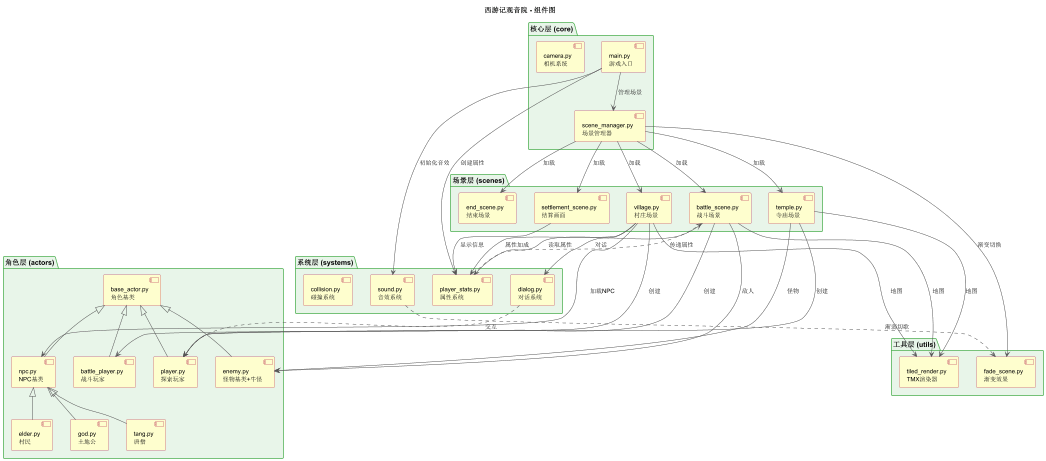
\includegraphics[width=0.9\textwidth]{figures/component_diagram.png}
    \caption{系统组件图}
    \label{fig:component}
\end{figure}

各层职责如下：

\begin{itemize}
    \item \textbf{核心层}：Game主类、场景管理器、相机系统，负责游戏初始化和主循环
    \item \textbf{角色层}：角色基类ActorBase、玩家Player/BattlePlayer、NPC基类NPCBase、怪物基类EnemyBase
    \item \textbf{系统层}：对话系统、属性系统、音效系统、碰撞系统
    \item \textbf{场景层}：场景基类SceneBase、村庄/寺庙/战斗/结算场景
    \item \textbf{工具层}：TMX渲染器、渐变效果
\end{itemize}

\subsection{类设计}

系统采用继承体系设计角色和场景类。

\begin{figure}[H]
    \centering
    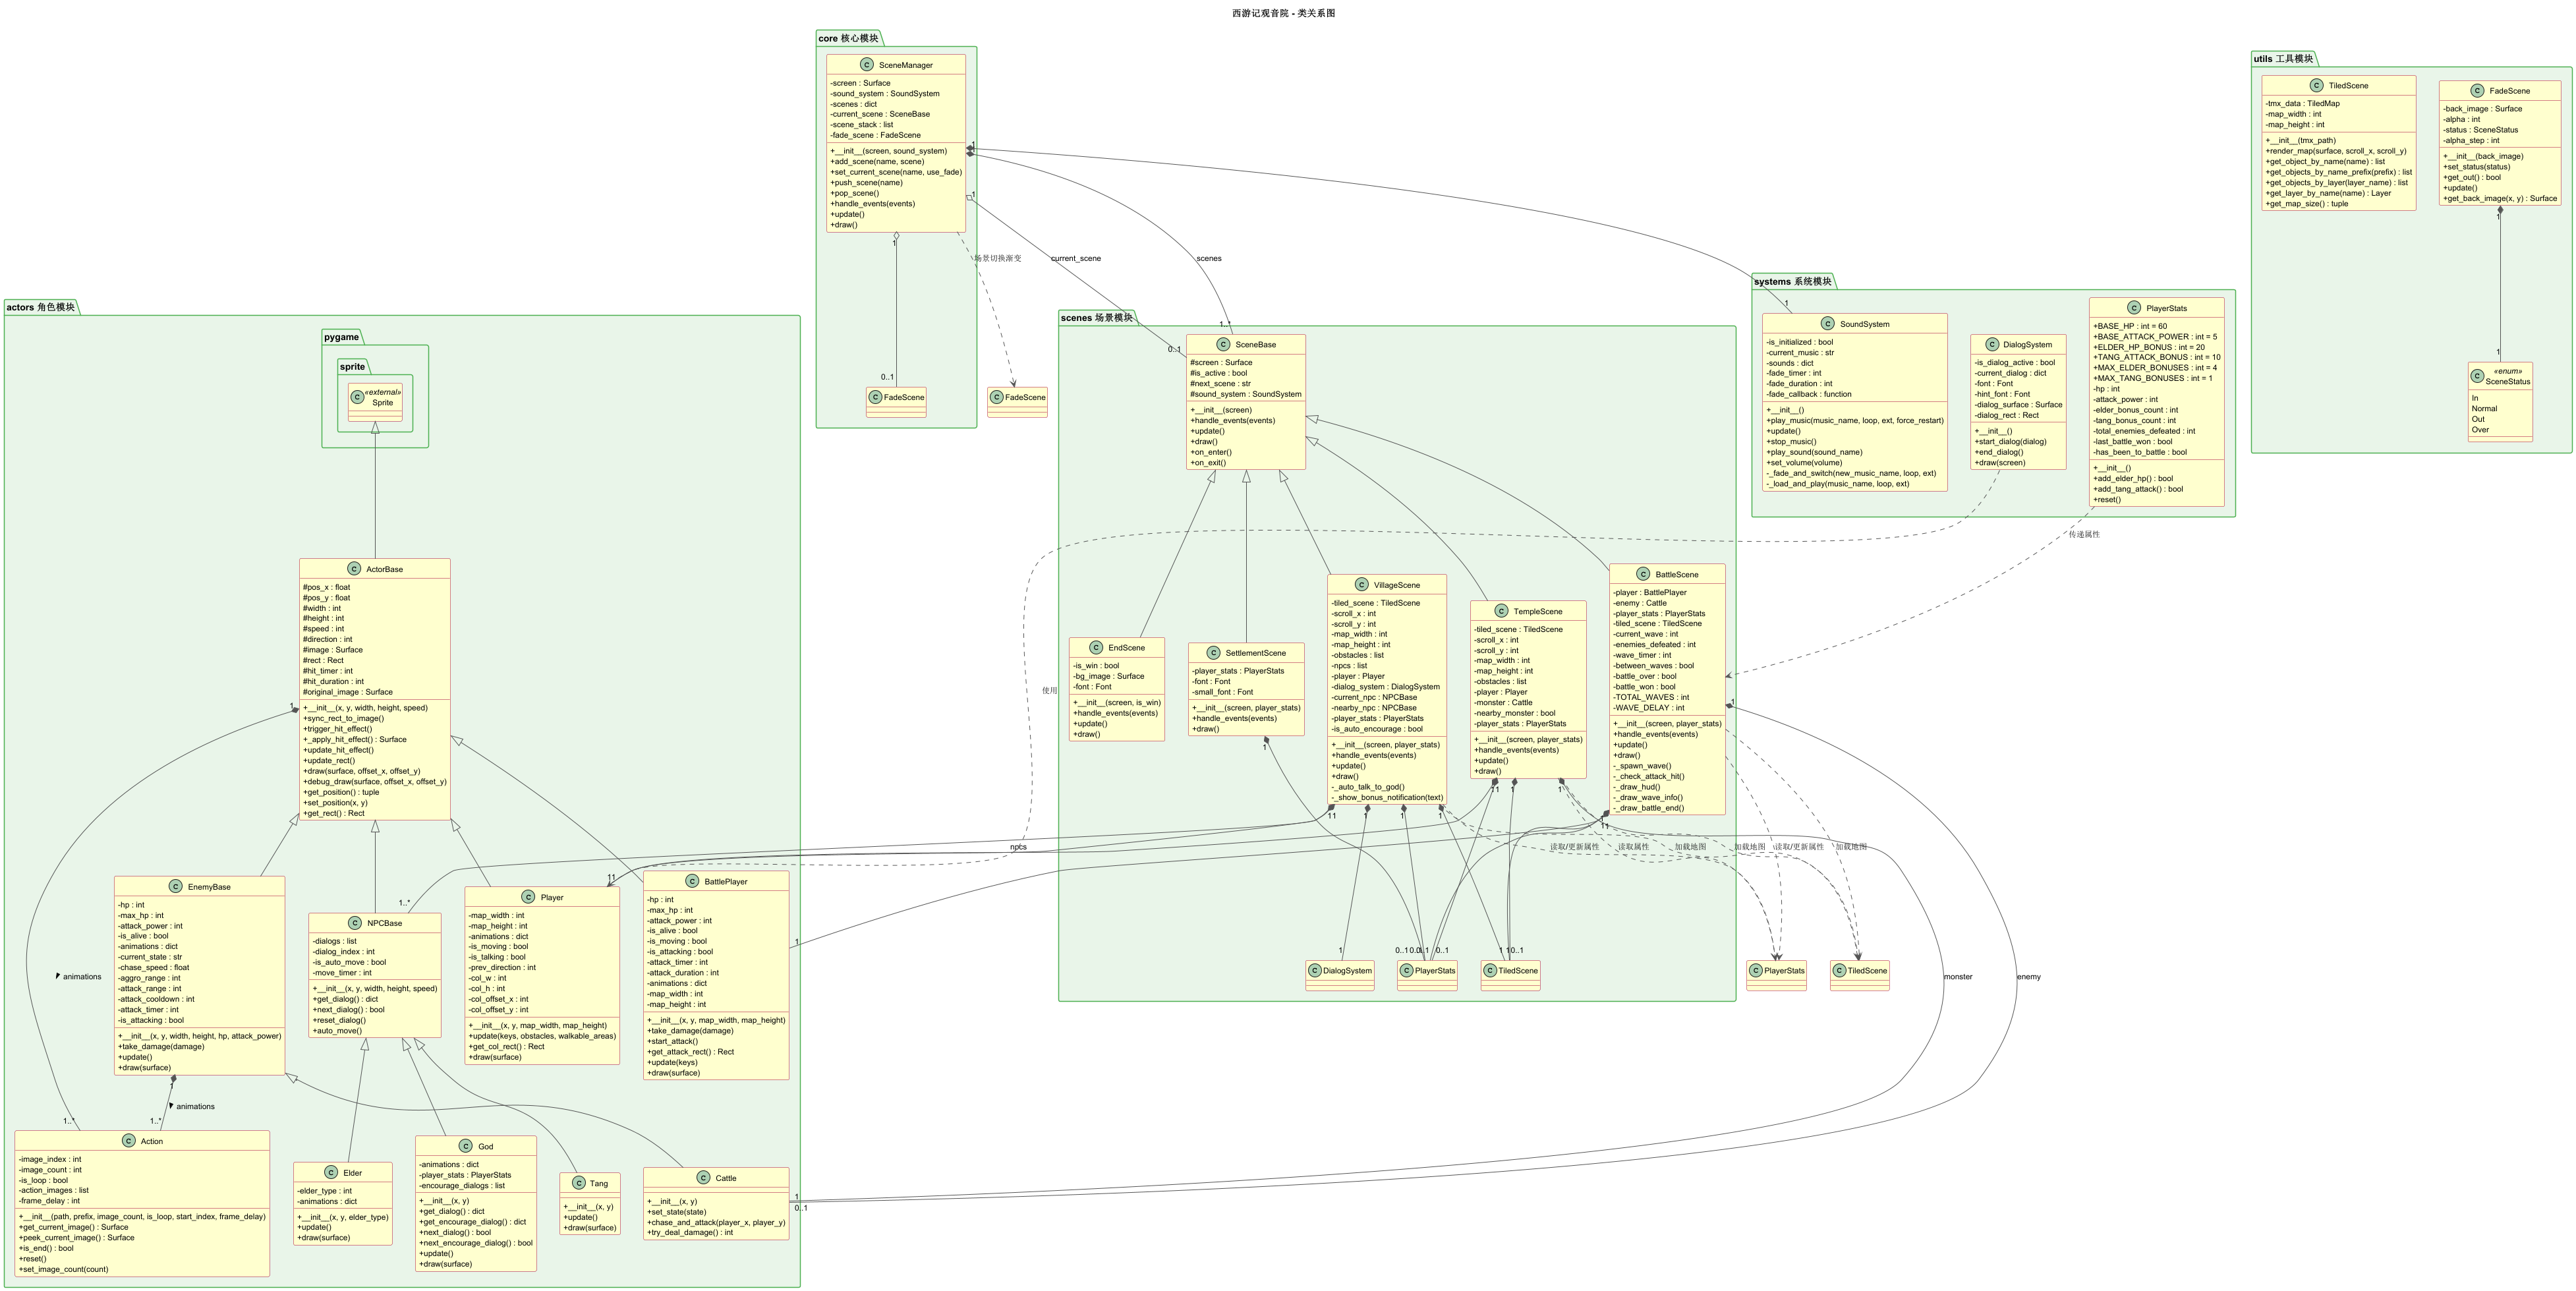
\includegraphics[width=0.95\textwidth]{figures/class_diagram.png}
    \caption{类关系图}
    \label{fig:class}
\end{figure}

核心类说明：

\begin{longtable}{>{\centering\arraybackslash}m{2.5cm}>{\centering\arraybackslash}m{2.5cm}>{\centering\arraybackslash}m{6cm}}
\caption{核心类说明} \label{tab:classes} \\
\toprule
\textbf{类名} & \textbf{所属模块} & \textbf{职责} \\
\midrule
\endfirsthead

\toprule
\multicolumn{3}{l}{续表} \\
\textbf{类名} & \textbf{所属模块} & \textbf{职责} \\
\midrule
\endhead

\midrule
\multicolumn{3}{r}{续下页} \\
\endfoot

\bottomrule
\endlastfoot

ActorBase & actors & 角色基类，管理位置、动画、受击效果 \\
Player & actors & 探索模式玩家，WASD移动 \\
BattlePlayer & actors & 战斗模式玩家，WASD+鼠标攻击 \\
NPCBase & actors & NPC基类，管理对话和自主移动 \\
EnemyBase & actors & 怪物基类，管理血量和追击AI \\
SceneBase & scenes & 场景基类，管理场景生命周期 \\
VillageScene & scenes & 村庄场景，含NPC交互和属性加成 \\
BattleScene & scenes & 战斗场景，实时战斗+波次系统 \\
PlayerStats & systems & 玩家属性管理，跨场景持久化 \\
SoundSystem & systems & 音效系统，含渐弱切歌 \\
\end{longtable}

\subsection{用例设计}

\begin{figure}[H]
    \centering
    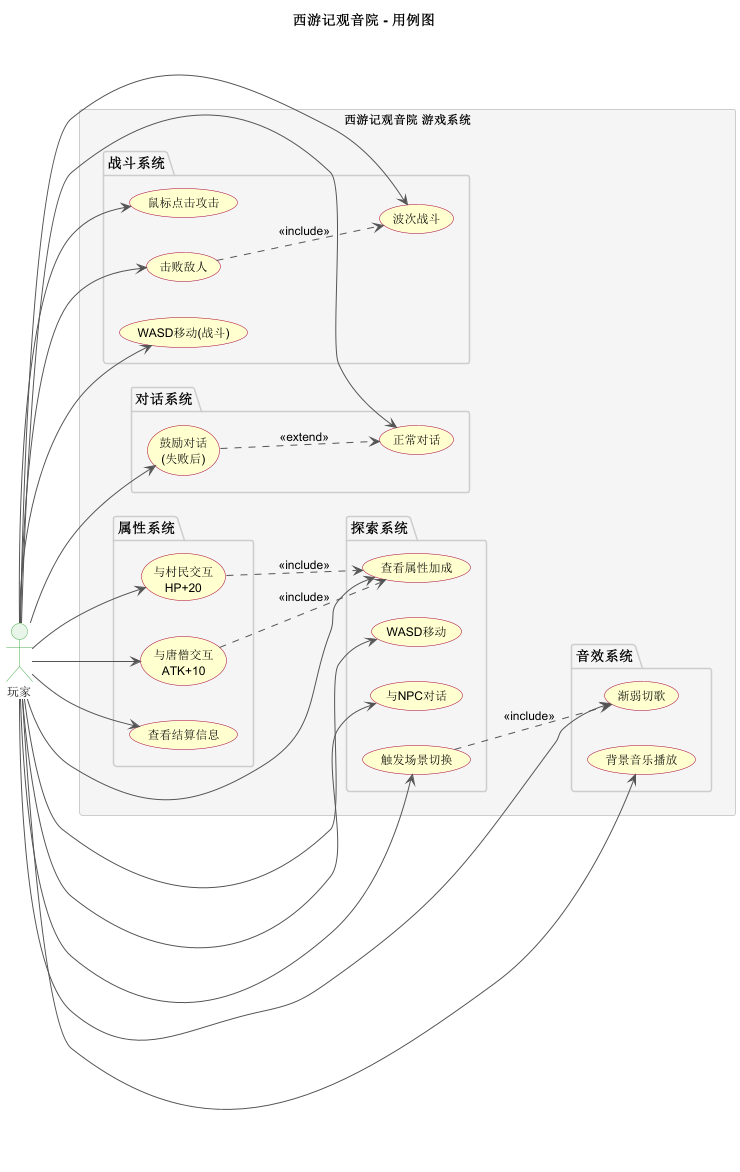
\includegraphics[width=0.95\textwidth]{figures/use_case_diagram.png}
    \caption{用例图}
    \label{fig:usecase}
\end{figure}

玩家与系统的交互关系：

\begin{longtable}{>{\centering\arraybackslash}m{2.5cm}>{\centering\arraybackslash}m{4cm}>{\centering\arraybackslash}m{5cm}}
\caption{用例说明} \label{tab:usecase} \\
\toprule
\textbf{用例} & \textbf{触发条件} & \textbf{系统响应} \\
\midrule
\endfirsthead

\toprule
\multicolumn{3}{l}{续表} \\
\textbf{用例} & \textbf{触发条件} & \textbf{系统响应} \\
\midrule
\endhead

\midrule
\multicolumn{3}{r}{续下页} \\
\endfoot

\bottomrule
\endlastfoot

WASD移动 & 按WASD键 & 玩家角色移动 \\
与NPC对话 & 靠近NPC按空格 & 显示对话框 \\
触发场景切换 & 土地公对话结束 & 渐变切换到寺庙 \\
鼠标点击攻击 & 鼠标左键点击 & 发起挥砍攻击 \\
击败敌人 & 敌人HP≤0 & 敌人死亡，波次切换 \\
与村民交互 & Elder对话结束 & HP+20 \\
与唐僧交互 & Tang对话结束 & ATK+10 \\
渐弱切歌 & 切换场景 & 当前音乐渐弱→新音乐播放 \\
\end{longtable}

\subsection{状态设计}

\subsubsection{战斗状态}

\begin{figure}[H]
    \centering
    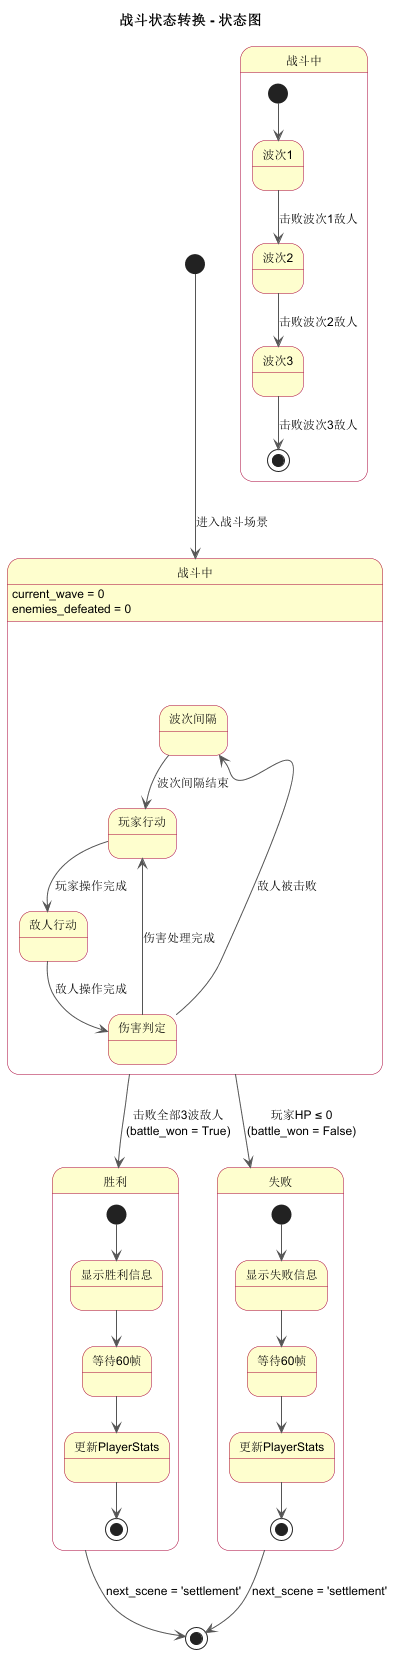
\includegraphics[width=0.8\textwidth, height=0.85\textheight, keepaspectratio]{figures/state_battle.png}
    \caption{战斗状态转换图}
    \label{fig:state_battle}
\end{figure}

\subsubsection{玩家状态}

\begin{figure}[H]
    \centering
    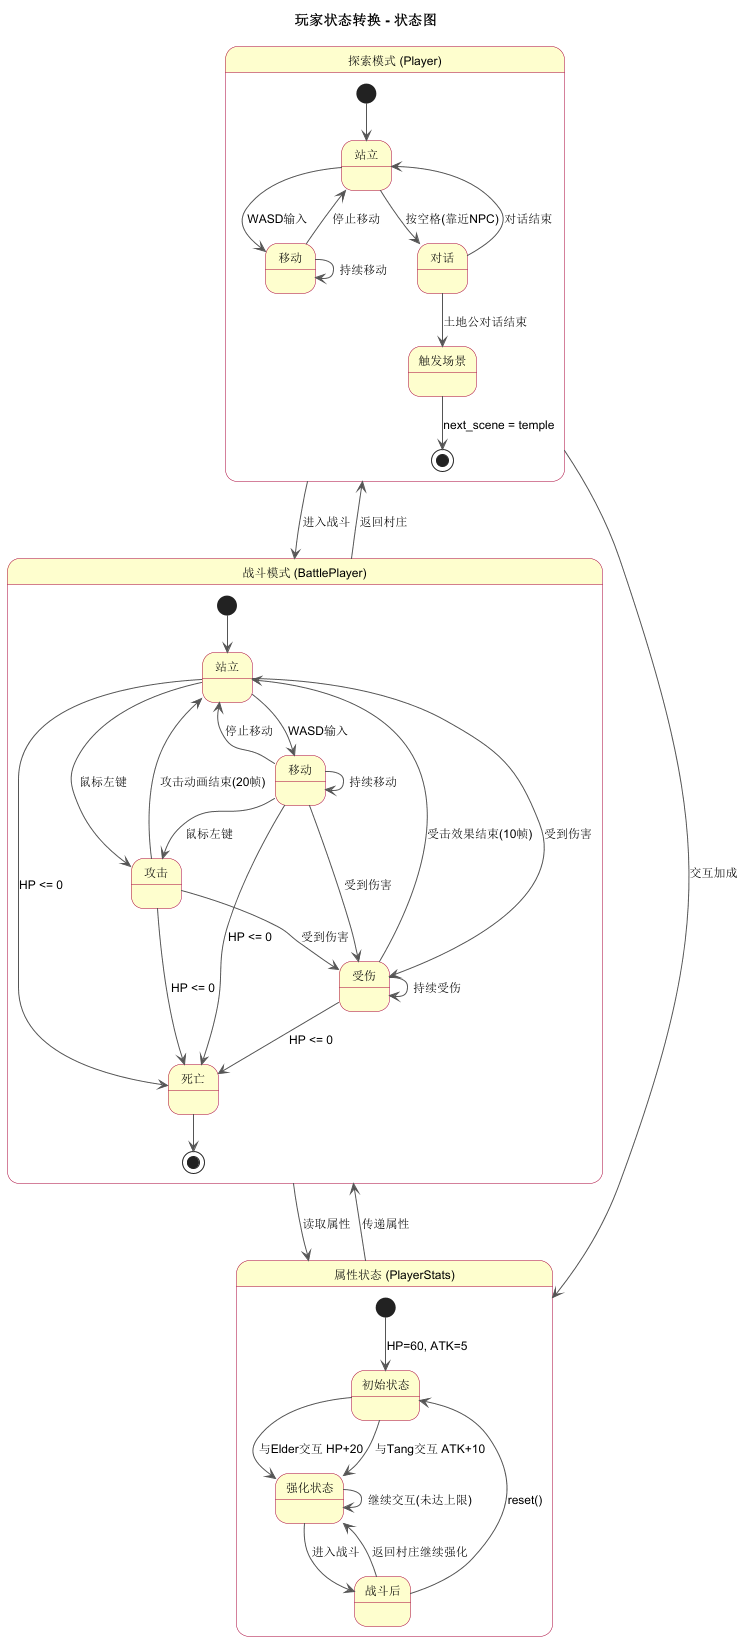
\includegraphics[width=0.9\textwidth, height=0.85\textheight, keepaspectratio]{figures/state_player.png}
    \caption{玩家状态转换图}
    \label{fig:state_player}
\end{figure}

\subsection{流程设计}

\subsubsection{实时战斗流程}

\begin{figure}[H]
    \centering
    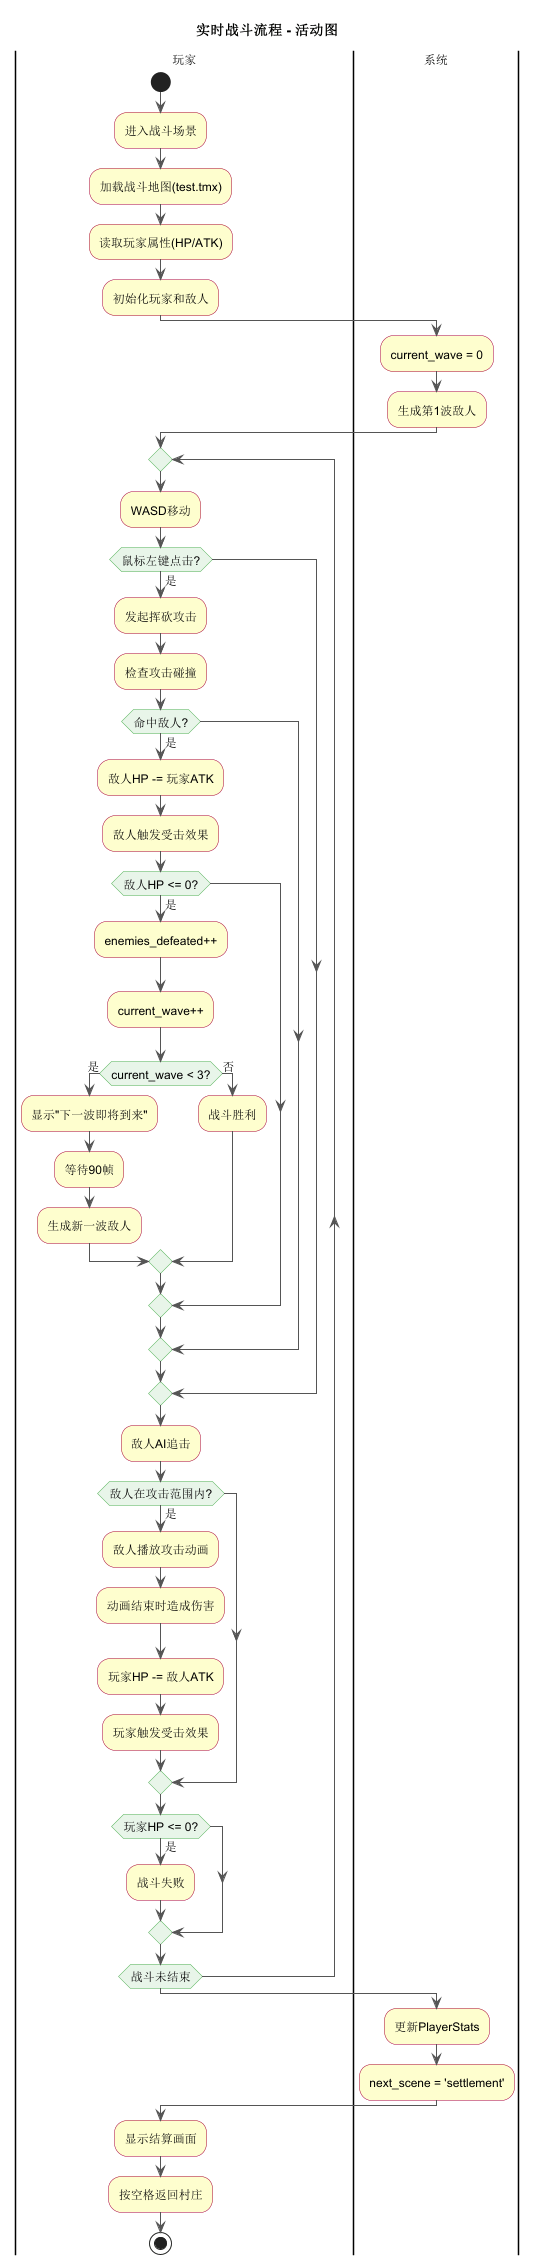
\includegraphics[width=0.6\textwidth, height=0.85\textheight, keepaspectratio]{figures/activity_battle.png}
    \caption{实时战斗活动图}
    \label{fig:activity_battle}
\end{figure}

\subsubsection{场景切换流程}

\begin{figure}[H]
    \centering
    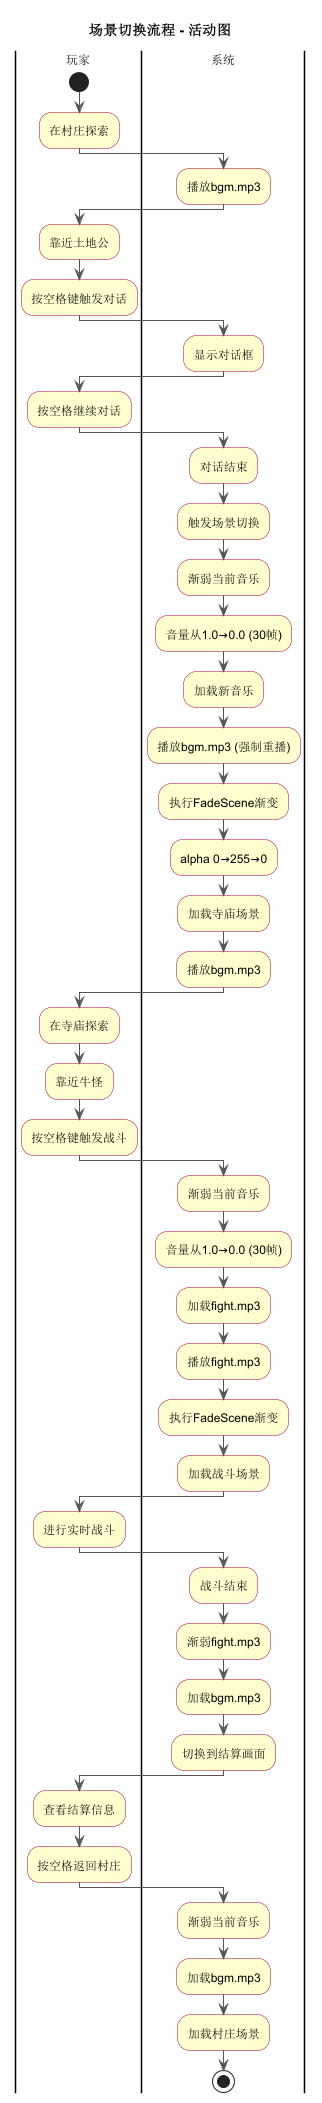
\includegraphics[width=0.5\textwidth, height=0.85\textheight, keepaspectratio]{figures/activity_scene_switch.png}
    \caption{场景切换活动图}
    \label{fig:activity_scene}
\end{figure}

\subsubsection{NPC对话交互}

\begin{figure}[H]
    \centering
    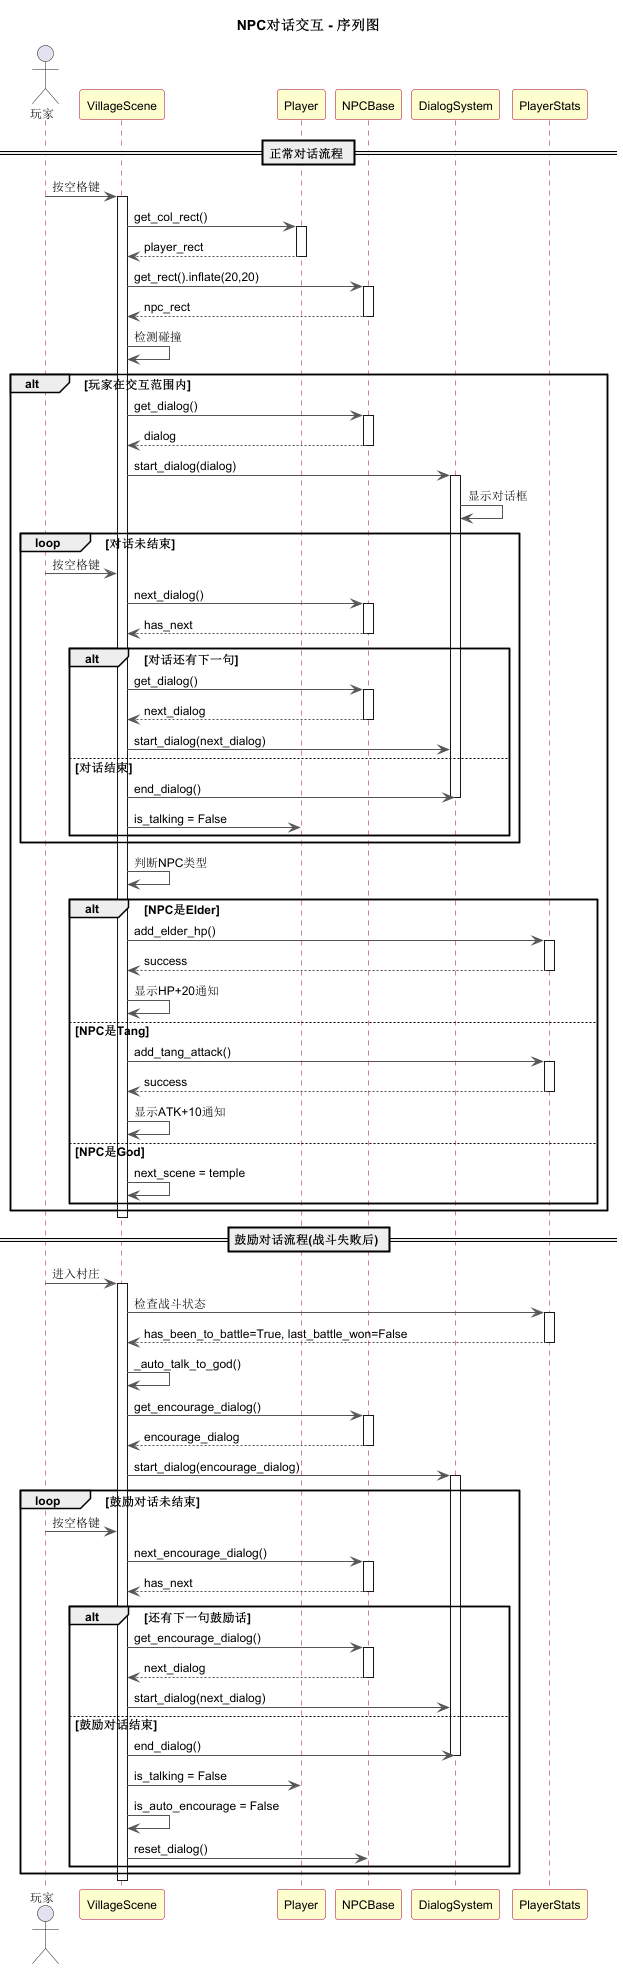
\includegraphics[width=0.85\textwidth, height=0.85\textheight, keepaspectratio]{figures/sequence_dialog.png}
    \caption{NPC对话序列图}
    \label{fig:seq_dialog}
\end{figure}

\subsubsection{战斗交互}

\begin{figure}[H]
    \centering
    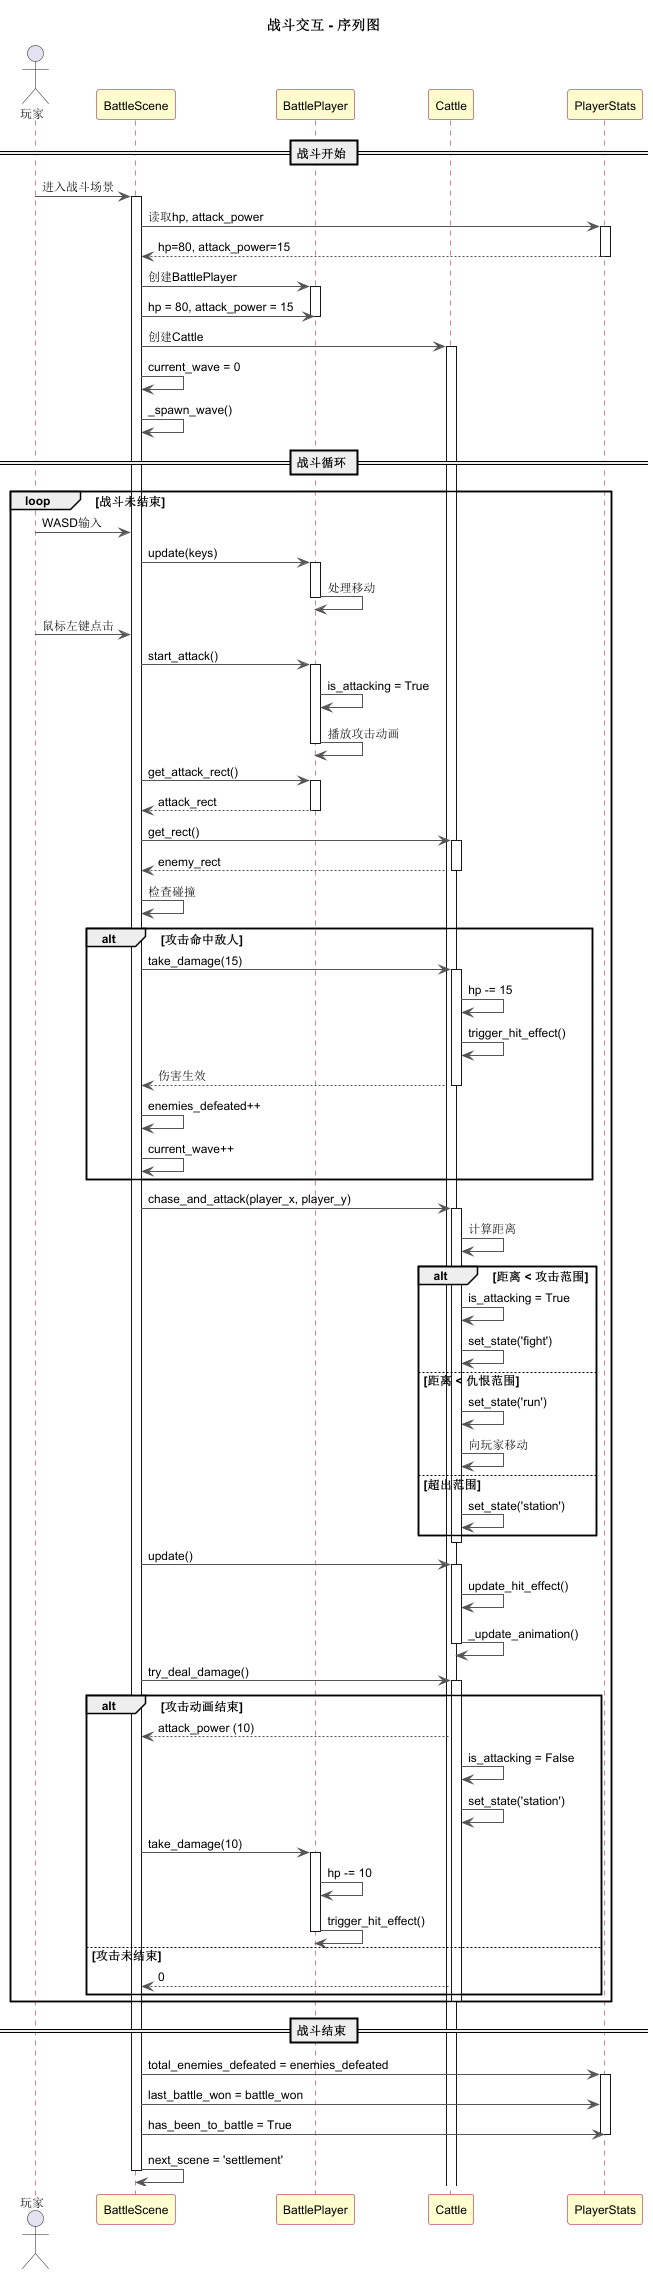
\includegraphics[width=0.9\textwidth, height=0.85\textheight, keepaspectratio]{figures/sequence_battle.png}
    \caption{战斗交互序列图}
    \label{fig:seq_battle}
\end{figure}

% ================================================================
% 五、数据设计
% ================================================================
\section{数据设计}

\subsection{资源文件}

\begin{longtable}{>{\centering\arraybackslash}m{2.5cm}>{\centering\arraybackslash}m{3.5cm}>{\centering\arraybackslash}m{5cm}}
\caption{资源文件清单} \label{tab:resources} \\
\toprule
\textbf{类型} & \textbf{路径} & \textbf{说明} \\
\midrule
\endfirsthead

\toprule
\multicolumn{3}{l}{续表} \\
\textbf{类型} & \textbf{路径} & \textbf{说明} \\
\midrule
\endhead

\midrule
\multicolumn{3}{r}{续下页} \\
\endfoot

\bottomrule
\endlastfoot

玩家精灵(探索) & resource/img/swk2/ & 孙悟空128帧PNG \\
玩家精灵(战斗) & resource/img/swk/ & 孙悟空16帧TGA \\
NPC精灵 & resource/img/elder/ & 村民TGA格式 \\
怪物精灵 & resource/img/cattle/ & 牛怪TGA格式 \\
土地公 & resource/img/god/ & 土地公4方向40帧 \\
地图文件 & resource/tmx/village1.tmx & 村庄地图 \\
地图文件 & resource/tmx/temple.tmx & 寺庙地图 \\
地图文件 & resource/tmx/test.tmx & 战斗地图（暂时） \\
字体文件 & resource/font/newfont.TTF & 中文字体 \\
背景音乐 & resource/sound/bgm.mp3 & 村庄/寺庙音乐 \\
战斗音乐 & resource/sound/fight.mp3 & 战斗音乐 \\
\end{longtable}

\subsection{TMX地图结构}

\begin{longtable}{>{\centering\arraybackslash}m{2.5cm}>{\centering\arraybackslash}m{2.5cm}>{\centering\arraybackslash}m{5.5cm}}
\caption{TMX地图图层结构} \label{tab:tmx} \\
\toprule
\textbf{图层名称} & \textbf{类型} & \textbf{说明} \\
\midrule
\endfirsthead

\toprule
\multicolumn{3}{l}{续表} \\
\textbf{图层名称} & \textbf{类型} & \textbf{说明} \\
\midrule
\endhead

\midrule
\multicolumn{3}{r}{续下页} \\
\endfoot

\bottomrule
\endlastfoot

backgroud & imagelayer & 背景图层 \\
actor & objectgroup & 玩家位置 (sun, tang) \\
elder & objectgroup & 村民NPC位置 (elder1\~4) \\
god & objectgroup & 土地公位置 \\
child & objectgroup & 儿童NPC位置 \\
obstacle & objectgroup & 障碍物碰撞区域 \\
road & objectgroup & 可行走区域 \\
\end{longtable}

\subsection{玩家属性配置}

\begin{longtable}{>{\centering\arraybackslash}m{3.5cm}>{\centering\arraybackslash}m{2cm}>{\centering\arraybackslash}m{5.5cm}}
\caption{玩家属性配置} \label{tab:player_attr} \\
\toprule
\textbf{属性} & \textbf{值} & \textbf{说明} \\
\midrule
\endfirsthead

\toprule
\multicolumn{3}{l}{续表} \\
\textbf{属性} & \textbf{值} & \textbf{说明} \\
\midrule
\endhead

\midrule
\multicolumn{3}{r}{续下页} \\
\endfoot

\bottomrule
\endlastfoot

BASE\_HP & 60 & 初始血量 \\
BASE\_ATTACK\_POWER & 5 & 初始攻击力 \\
ELDER\_HP\_BONUS & 20 & 每次与村民交互增加血量 \\
TANG\_ATTACK\_BONUS & 10 & 每次与唐僧交互增加攻击力 \\
MAX\_ELDER\_BONUSES & 4 & 最多4个村民可交互 \\
MAX\_TANG\_BONUSES & 1 & 1个唐僧可交互 \\
\end{longtable}

\subsection{战斗配置}

\begin{longtable}{>{\centering\arraybackslash}m{3.5cm}>{\centering\arraybackslash}m{2cm}>{\centering\arraybackslash}m{5.5cm}}
\caption{战斗配置} \label{tab:battle_config} \\
\toprule
\textbf{属性} & \textbf{值} & \textbf{说明} \\
\midrule
\endfirsthead

\toprule
\multicolumn{3}{l}{续表} \\
\textbf{属性} & \textbf{值} & \textbf{说明} \\
\midrule
\endhead

\midrule
\multicolumn{3}{r}{续下页} \\
\endfoot

\bottomrule
\endlastfoot

TOTAL\_WAVES & 3 & 总波次数 \\
WAVE\_DELAY & 90 & 波次间隔帧数（约2.25秒） \\
敌人追击速度 & 1.5 & 比玩家慢（玩家速度4） \\
敌人仇恨范围 & 300px & 开始追击的距离 \\
敌人攻击范围 & 40px & 开始攻击的距离 \\
敌人攻击冷却 & 60帧 & 攻击间隔（约1.5秒） \\
挥砍范围 & 60px & 玩家攻击距离 \\
挥砍宽度 & 80px & 玩家攻击宽度 \\
\end{longtable}

% ================================================================
% 六、附录
% ================================================================
\section{附录}

\subsection{项目结构}

\begin{lstlisting}[language={},caption={项目目录结构}]
journey_to_the_west/
├── main.py              # 游戏入口
├── config.py            # 全局配置
├── core/
│   ├── game.py          # Game主类
│   ├── camera.py        # 相机系统
│   └── scene_manager.py # 场景管理器
├── actors/
│   ├── action.py        # Action 动画行为类
│   ├── base_actor.py    # ActorBase 角色基类
│   ├── player.py        # Player 孙悟空(探索)
│   ├── battle_player.py # BattlePlayer 孙悟空(战斗)
│   ├── npc.py           # NPC基类
│   ├── elder.py         # Elder 村民
│   ├── god.py           # God 土地公
│   ├── tang.py          # Tang 唐僧
│   └── enemy.py         # EnemyBase + Cattle
├── systems/
│   ├── dialog.py        # 对话系统
│   ├── player_stats.py  # 玩家属性系统
│   ├── sound.py         # 音效系统
│   └── collision.py     # 碰撞系统
├── scenes/
│   ├── base_scene.py    # SceneBase 场景基类
│   ├── village.py       # 村庄场景
│   ├── temple.py        # 寺庙场景
│   ├── battle_scene.py  # 战斗场景
│   ├── settlement_scene.py # 结算画面
│   └── end_scene.py     # 结束场景
├── utils/
│   ├── tiled_render.py  # TMX渲染器
│   └── fade_scene.py    # 渐变效果
└── resource/            # 资源文件
\end{lstlisting}

\end{document}
